%\documentclass[journal]{IEEEtran}
\documentclass[]{article}

% \renewcommand\IEEEkeywordsname{Keywords}

\usepackage{graphicx}
\usepackage{rotating}
\usepackage{adjustbox}
\usepackage{blindtext}
\graphicspath{ {images/} }
\usepackage{tabularx}
\usepackage{caption}
\usepackage{pdfpages}
\usepackage{amsmath}
\usepackage{subcaption}
\usepackage{float}
\usepackage{xcolor,bytefield}
\usepackage{color,soul}
\usepackage{fancyhdr}
\pagenumbering{arabic}
\usepackage[margin=1in]{geometry}
\usepackage{hyperref}
\bibliographystyle{IEEEtran}

\providecommand{\keywords}[1]{\textbf{\textit{Keywords:}} #1}
\newcommand{\colorbitbox}[3]{%
	\sbox0{\bitbox{#2}{#3}}%
	\makebox[0pt][l]{\textcolor{#1}{\rule[-\dp0]{\wd0}{\ht0}}}%
	\bitbox{#2}{#3}%
}

\pagestyle{fancy}
\fancyhf{}
\rhead{AJS Systems}
\lhead{COMPSYS701 - Advanced Digital Systems Design}
\cfoot{\thepage}


\begin{document}
	\markboth{COMPSYS701 - Advanced Digital Systems Design}{}
	
	\begin{titlepage}
		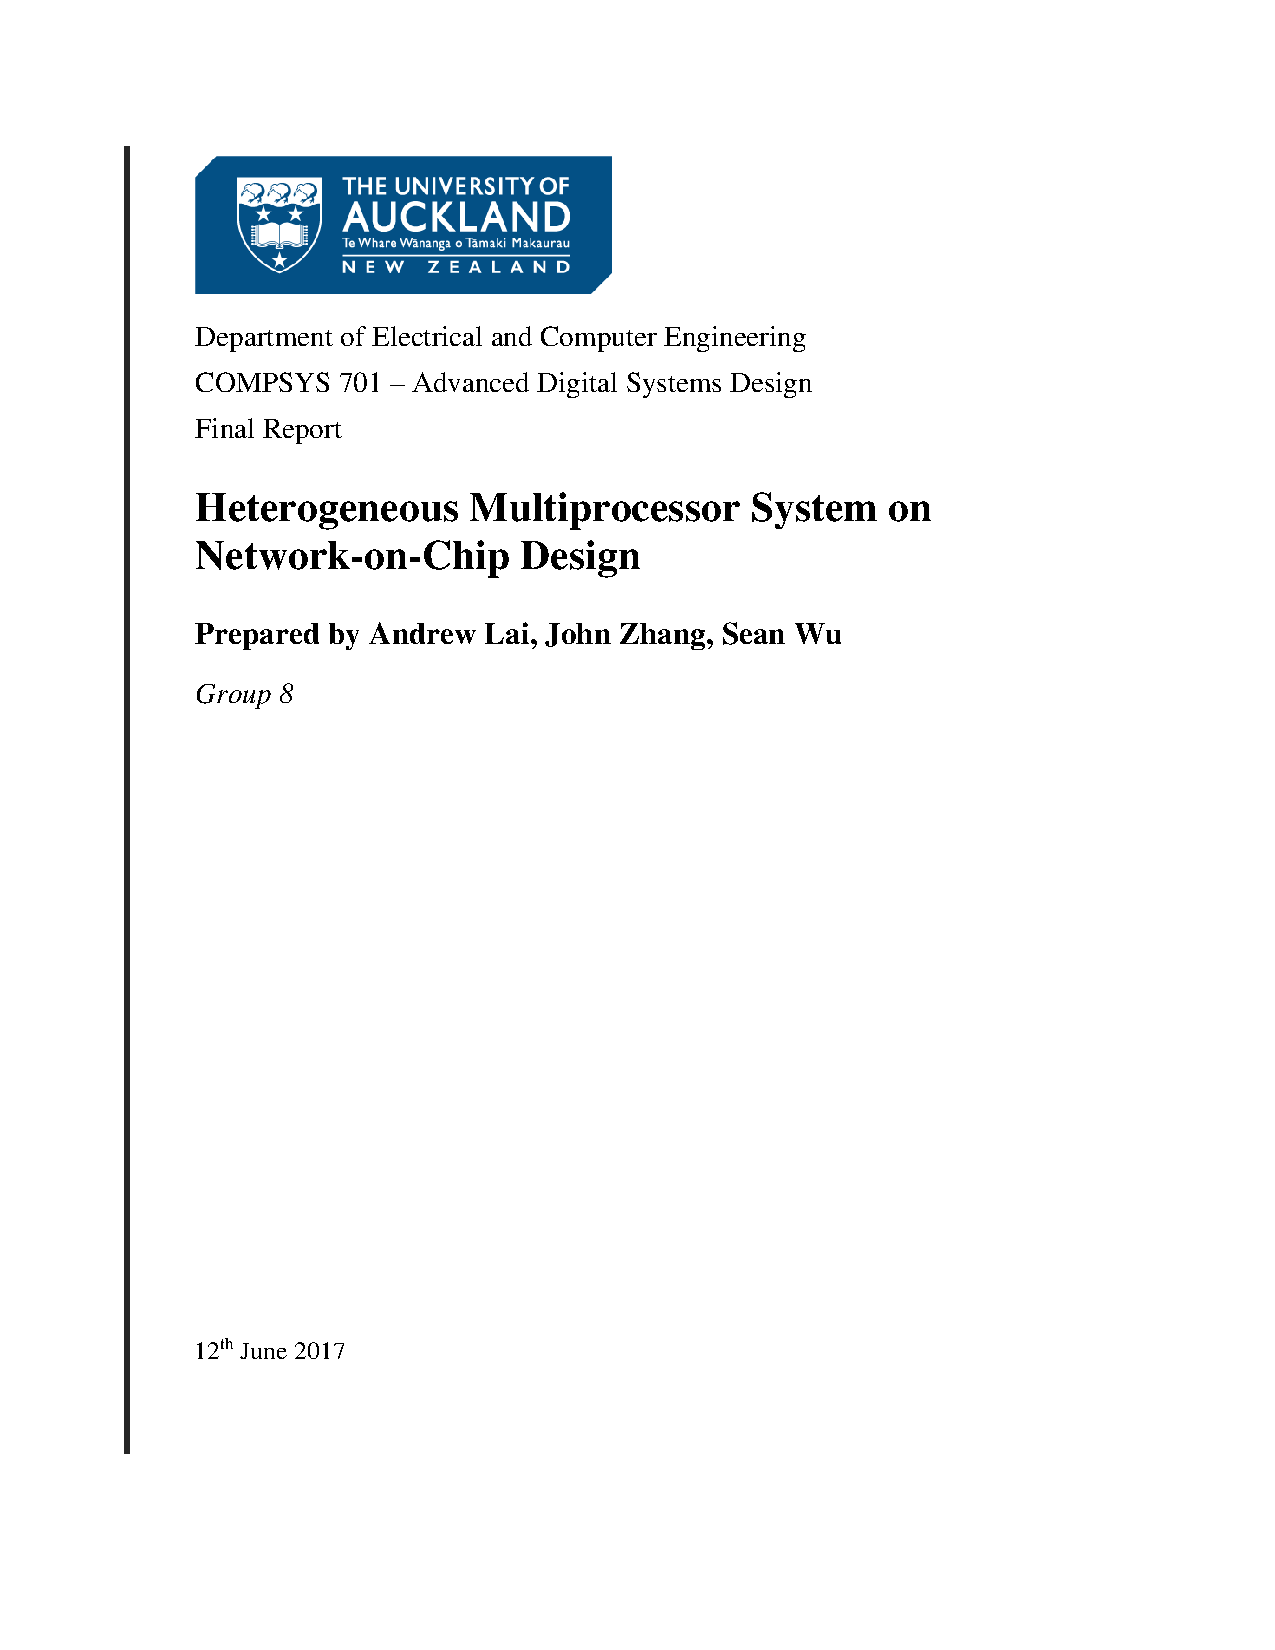
\includepdf[pages={1}]{title_page.pdf}
	\end{titlepage}
	\tableofcontents
	\setcounter{page}{1}
	
	\title{\huge \textbf{Heterogeneous Multiprocessor System on Network-on-Chip Design}}
	\author{Group 8 (AJS) - Andrew Lai \texttt{(klai054)}, John Zhang \texttt{(szha215)}, Shiyang Wu \texttt{(swu145)} \\Department of Electrical and Computer Engineering, University of Auckland, New Zealand}
	
	\maketitle
	
	\begin{abstract}
		With Moore’s Law becoming more difficult to achieve, multi-core or multiprocessor systems are becoming more popular ways to improve performance rather than focusing on architecture size or maximum frequency for single-core chips. This report presents a heterogeneous multiprocessor system design using the Network-on-Chip approach implemented in System-on-Chip, including designing a new hardware acceleration processor, network interfaces and integrating them alongside processors using the SystemJ programming language -- which can run system-level and Java programmes on hardware-accelerated Jave Optimised Processors (JOP).
	\end{abstract}
	
	%     \begin{IEEEkeywords}
	%         Processor design; Network-on-chip 
	%     \end{IEEEkeywords}
	
	\keywords{Processor design, Network-on-chip}
	
	\section{Introduction}
	
	There has been an increased demand on computation requirements and functionality, and it has become troublesome to continue the advancements in the capabilities of a single-core processor chip. An alternative attempt to fulfil this demand is the development of a multi-core system. There has been a development of advanced multicore system-on-chip which provide a very powerful execution platform which can either be comprised of homogenous, comprised of many cores of the same type, or heterogeneous, by mixing different types of cores. As there is an increased number of processor cores, the importance and emphasis of parallelism and time predictability become important factors to consider when trying to make sure that the platform is effectively executed.
	\par 
	This project report will present a take on developing a System-on-Chip (SoC) in which is based on the notion of the Network-on-Chip (NoC) concept. This will feature the development of a prototype SoC which allows for computer systems designers to program software or hardware solutions for embedded systems. This system-on-chip is to be a heterogeneous execution platform with different types of cores connected together; the resulting product is the called the ADD-HSoC (which stands for Advanced Digital Design - Heterogenous System on Chip). The system will utilise the access distribution method of Time-Division Multiple Access -- Multistage Interconnection Network (TDMA-MIN) to achieve correct execution, with high bandwidth and with guaranteed latency for the prevention of packet interleaving when communicating between multiple cores.
	
	
	The project is to be broken into phases, whereby each phase is a milestone which marks great strides in the development of the ADD-HSoC project. These phases entail: the design of processors, Application Specific Processor and Reactive Coprocessor from scratch to be placed in the NoC, the integration of the processors so that it is capable of inter-communication and a SystemJ application to demonstrate the functionalities of the ADD-HSoC.
	\newpage
	\subsection{Project Phases}
	\begin{enumerate}
		\item Phase One: General and Application Specific Processor Design
		\begin{itemize}
			\item Design of ReCOP processor (AJS)
			\item Design of ASP and its network interface
		\end{itemize}
		
		\item Phase Two: Network Interface modifications
		\begin{itemize}
			\item Program development for JOPs
			\item Adaptation of JOP Network Interface (JNI) to support communication with ASP
			\item Integration of JOP and ASP using TDMA-MIN
			\item Integration of AJS ReCOP and JOP using TDMA-MIN
		\end{itemize}
		
		\item Phase Three: ADD-HSoC Integration
		\begin{itemize}
			\item Integration of all components into full blown ADD-HSoC
			\item SystemJ program demonstrating ADD-HSoC execution
		\end{itemize}
		
	\end{enumerate}
	
	
	
	\section{Network-on-Chip Structure}
	
	\subsection{Architecture Overview}
	The ADD-HSoC is a network-on-chip that consists of three different types of processors interconnected to execute SystemJ. The three main processor cores types are ReCOP, JOP and ASP. Each of these processors is capable of stand-alone execution and has its own instruction set architecture each unique to its own. Each type processor is capable of communicating with each other, however, with the introduction of TDMA-MIN, the identity of each packet will not be sufficient to communicate in a multi-core system. As a result, either modification to the processor or an external module must be made to adapt to a specific port in the TDMA-MIN system. The choice is to make network interfaces unique to each core to make the communications possible between cores. \par 
	
	\begin{figure}[H]
		\centering
		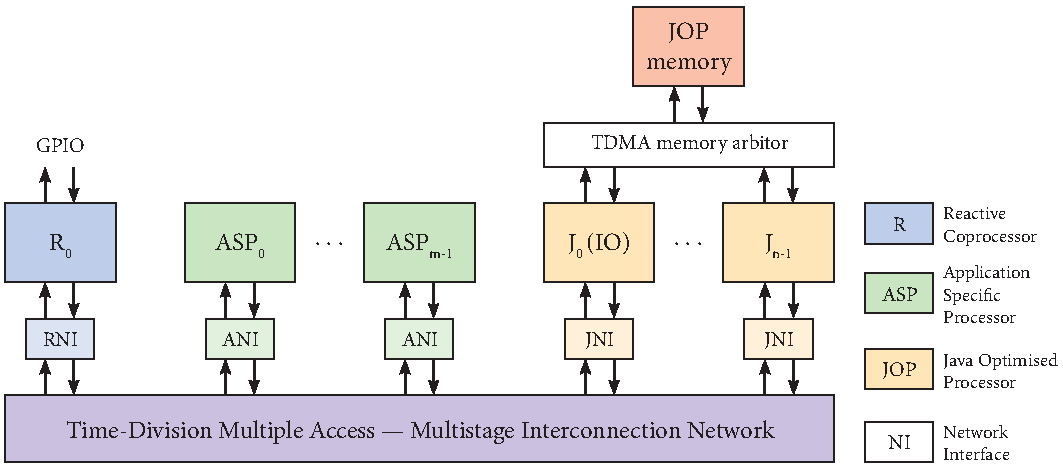
\includegraphics[width = 5.5in]{noc_block_diagram}
		\caption{Top-level diagram of TDMA-MINoC}
		\label{fig:noc_block}
	\end{figure}
	
	
	The overall structure for as seen in Fig. \ref{fig:noc_block}, is the protocol of interconnection for the multicore system. Each processor core connects to its own network interface and each network interface is connected to the TDMA-MIN. With this, the project initially started with a given JOP. JOP network interface, ReCOP and ReCOP network interface designs for a head start on the project, each one modified during the project to accommodate for the ADD-HSoC configuration.
	
	\subsection{Configuration}
	
	The configuration and function of the ADD-HSoC are for the system to feature multi-core intercommunication; this will ultimately be used to execute SystemJ applications. When SystemJ is compiled and programmed into the system, it is separated into their respective cores for computation. Each SystemJ application can be described with AGRC graphs, to capture the fact there are two different types of computation that can be simply described as a set of control and data computations \cite{Malik2008}. This is where it can be specified that the ReCOP will execute control logic such as actions or decisions, and the JOP executes data computations like Java code functionality. This has already been developed where ReCOP Instruction Set Architecture (ISA) and Java have been made to be placed into their respective cores, the new aspect to the ADD-HSoC is to bring in an Application Specific Processor (ASP) to assist the JOP, much like an external hardware extension where the programmer is able to invoke the ASP if need be. \par 
	
	The execution of SystemJ can be extended to multiple ReCOPs, JOPs or ASPs to further catalyse computations for the execution platform and can be easily specified with the ADD-HSoC upon compilation. The top-level configuration file has been edited to accommodate for the addition of the new processor type in the system, the ASP, and a flag to choose between the ReCOP designs (v2 -- provided, or AJS -- designed). The number of ASPs can be up to 12, see Section \ref{sec:asp_data_format} for details.
	
	
	\section{Reactive Coprocessor (AJS)}
	The ReCOP designed by AJS is inspired by the MIPS multicycle implementation. This is chosen partially due to how each distinct part of the processor can be easily taken apart to be debugged and tested, using simulations with tools such as ModelSim to verify the functional correctness. The priority would be to ensure the functionality of executing instructions over efficient or fast processing. With that being said, the multicycle implementation is still open to further developments to make fast execution of instructions, such as pipelining cycles. \par 
	
	\begin{figure}[H]
		\centering
		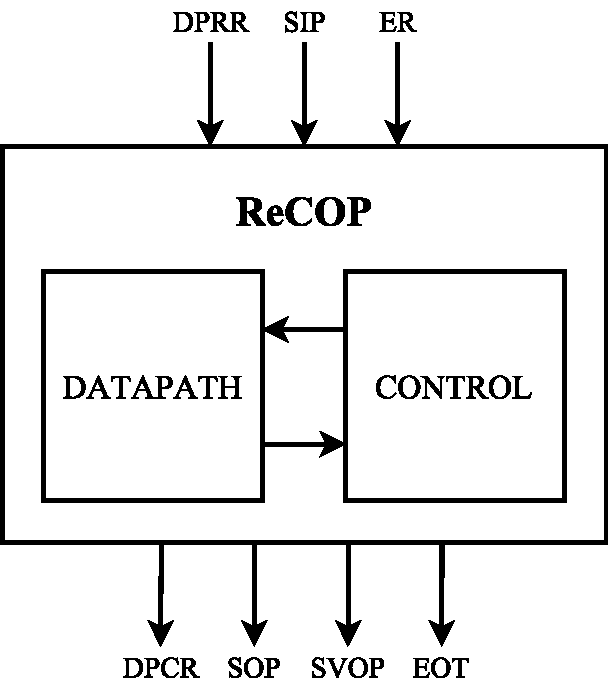
\includegraphics[width = 2.5in]{recop_block_diagram}
		\caption{Top-level diagram of ReCOP\_AJS}
		\label{fig:recop_block}
	\end{figure}
	
	The design for the ReCOP is broken down into two main components, the datapath and the control unit as illustrated in Fig. \ref{fig:recop_block}. The datapath is as the name implies contains all data components where data transfers in registers and memory are done. The datapath will rely on the control unit to control the dataflow within the ReCOP. The control unit as usual with multicycle implementation is with the use of a finite state machine to compute specific instructions.
	
	\subsection{Control Unit}
	The instructions of the ReCOP is broken down into its specific cycles of execution to for the multicycle implementation. As such, the instructions have been categorised to make sure the control unit’s finite state machine has a set of defined stages of control. The following is the categorisation of the ReCOP instruction set architecture.
	
	\subsubsection{ISA Categories}
	\begin{itemize}
		\item C-Type (Computation)
		\begin{itemize}
			\item \texttt{AND}, \texttt{OR}, \texttt{SUB}, \texttt{SUBV} and \texttt{MAX} 
		\end{itemize}
		
		\item L-Type (Load Register)
		\begin{itemize}
			\item \texttt{LDR}, \texttt{LER}, \texttt{SSVOP}, \texttt{LSIP} and \texttt{SSOP}
		\end{itemize}
		
		\item S-Type (Store Memory)
		\begin{itemize}
			\item \texttt{STR} and \texttt{STRPC}
		\end{itemize}
		
		\item JUMP Type
		\begin{itemize}
			\item \texttt{JMP}, \texttt{PRESENT} and \texttt{SZ}
		\end{itemize}
		\item D-Type (Data Call)
		\begin{itemize}
			\item \texttt{DCALLBL} and \texttt{DCALLNB}
		\end{itemize}
		
		\item F-Type (Flag Clear or Set)
		\begin{itemize}
			\item \texttt{CLFZ}, \texttt{CER}, \texttt{CEOT} and \texttt{SEOT}
		\end{itemize}
		
		
	\end{itemize}
	
	
	
	\subsubsection{FSM Refinement}
	
	
	The ReCOP follows a simple categorisation of states, they are as follows: Instruction Fetch and Decode, Execution of Instruction and Data call Result service routine. These are illustrated in Fig. \ref{fig:recop_fsm}. Each section is further broken down to ensure the correctness of execution.
	\begin{itemize}
		\item \emph{Instruction Fetch and Decode} \par
		The instruction fetch (\texttt{IF1}) is invoked and to set the PC to point to the next program memory address. This will fetch for the upper 16bit of the instruction, a stall state (\texttt{IF1S}) is in place to wait for synchronous register and memory to be stored. Then the instruction is decoded (\texttt{ID1}) and sent to the control unit to decipher if the lower 16 bits is needed to be used for the instruction (i.e. operand for immediate and direct addressing mode). While in this state, the operand is already prefetched in this state whether it is needed or not. If it is required, the control will set the PC to point to the next program memory address (\texttt{IF2} and \texttt{ID2}).
		
		\item \emph{Execution of Instruction} \par 
		The control unit will decide what the processor will do with the datapath based on what the instruction type is. The states are labelled with specific names to make it clear as to what sort of datapath controls it would require. The following is the breakdown of the execution states:
		\begin{itemize}
			\item \texttt{EX}: If the instruction uses the ALU
			\item \texttt{MA}: If memory access is needed to be loaded in the register
			\item \texttt{LR}: If register is loaded
			\item \texttt{SM}: If data is stored into memory
			\item \texttt{JP}: If a change in PC with jump or conditional
			\item \texttt{NOOP}: If no operation
			\item \texttt{DC}, \texttt{DCS}, \texttt{DCC}: If data call is executed. \texttt{DC} invokes the data call, \texttt{DCS} stalls for the synchronous store of the \texttt{DPCR}. \texttt{DCC} clears the \texttt{DPCR} so the call is not up for more than one clock cycle and executed multiple times. The state is also the loop state for blocking datacalls
		\end{itemize}
		
		\item \emph{Data call Result service routine} \par 
		This is a check on \texttt{DPRR} (\texttt{irq} bit of \texttt{DPRR} bit 1, shown in Fig. \ref{fig:recop_data_call_result_packet}), for a result from the NoC. This will then run the store of the result into memory writeback address or into register zero depending on if the datacall was nonblocking or blocking respectively. If there is no result to be processed, the ReCOP will execute the next instruction, entering the Instruction Fetch and Decode (\texttt{IF1}) state.
		
	\end{itemize}
	
	\begin{figure}[H]
		\centering
		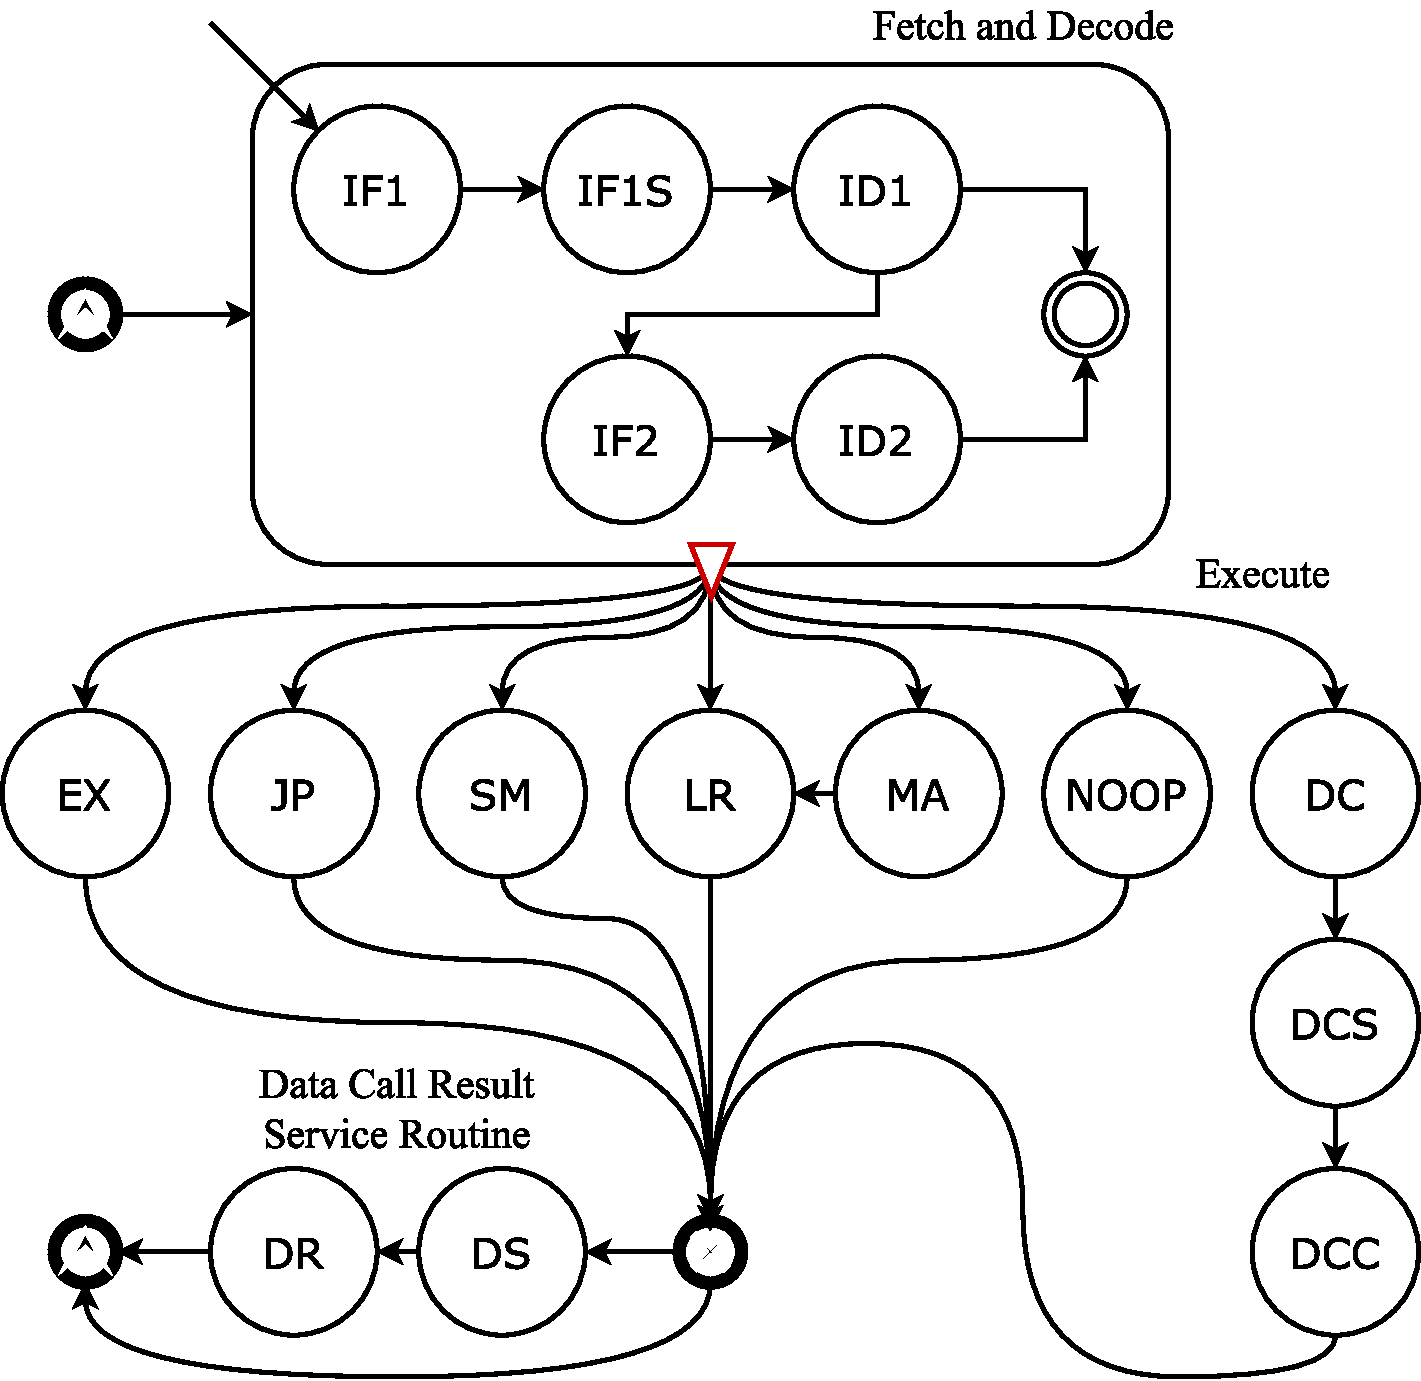
\includegraphics[width = 4in]{recop_control_fsm}
		\caption{Control Unit FSM of ReCOP\_AJS}
		\label{fig:recop_fsm}
	\end{figure}
	
	\newpage
	
	\subsection{Data Format}
	
	\begin{figure}[H]
		\centering
		\captionsetup{justification=centering,margin=2cm}
		\begin{bytefield}[endianness=big,boxformatting={\centering},
			bitwidth=1em,bitheight=8mm]{32}
			\bitheader{0-31} \\
			\bitbox{2}{{\small AM}}
			\bitbox{6}{{\small Opcode}} &
			\bitbox{4}{\small Rz} &
			\bitbox{4}{\small Rx} &     
			\bitbox{16}{Operand} & 
		\end{bytefield}
		\caption{ReCOP\_AJS Instruction Format}
		\label{fig:recop_instruction_packet}
	\end{figure}
	
	Instructions for the ReCOP are broken down into either 32 bits or 16 bits depending if the instruction will require an operand or not respectively (shown in Fig. \ref{fig:recop_instruction_packet}). The addressing mode (AM) is what will decide if the operand is needed.
	
	
	
	\begin{figure}[H]
		\centering
		\captionsetup{justification=centering,margin=2cm}
		\begin{bytefield}[endianness=big,boxformatting={\centering},
			bitwidth=1em,bitheight=8mm]{32}
			\bitheader{0-31} \\
			\bitbox{1}{\rotatebox{90}{\tiny valid}}
			\bitbox{1}{\rotatebox{90}{\scalebox{.5}{Legacy(0)}}} &
			\colorbitbox{lightgray}{2}{\scalebox{.57}{Unused}} & 
			\bitbox{4}{\small JOP ID} &
			\bitbox{8}{\small Clock-domain ID} &     
			\bitbox{16}{Address to Java Method} & 
		\end{bytefield}
		\caption{ReCOP\_AJS Data-call Packet}
		\label{fig:recop_data_call_packet}
	\end{figure}
	
	\begin{figure}[H]
		\centering
		\captionsetup{justification=centering,margin=2cm}
		\begin{bytefield}[endianness=big,boxformatting={\centering},
			bitwidth=1em,bitheight=8mm]{32}
			\bitheader{0-31} \\
			\bitbox{1}{\rotatebox{90}{\tiny valid}}
			\bitbox{1}{\rotatebox{90}{\scalebox{.5}{Legacy(0)}}} &
			\bitbox{6}{\small ReCOP ID} & 
			\bitbox{12}{\small Writeback Address} &
			\colorbitbox{lightgray}{10}{\small Unused} &     
			\bitbox{1}{\rotatebox{90}{\tiny IRQ(1)}} &
			\bitbox{1}{\rotatebox{90}{\tiny Result}}
		\end{bytefield}
		\caption{ReCOP\_AJS Data-call Result Packet}
		\label{fig:recop_data_call_result_packet}
	\end{figure}
	
	Data calls (shown in Fig. \ref{fig:recop_data_call_packet} and Fig. \ref{fig:recop_data_call_result_packet}) by the ReCOP to the JOP and vice versa in the ADD-HSoC leave the legacy bit to be set to always be 0. The packet also specifies the JOP or ReCOP IDs and not the port destination as the network interfaces will handle the aggregation of packets to their ports.
	
	
	\newpage
	\enlargethispage{2in}
	
	\subsection{Datapath}
	
	
	\begin{figure}[H]
		\begin{adjustbox}{addcode={\begin{minipage}{\width}}{\caption{%
							ReCOP\_AJS Datapth.
						}\label{fig:reco_datapath}\end{minipage}},rotate=-90,center}
			\hspace*{-0.65in}
			\vspace*{0.65in}
			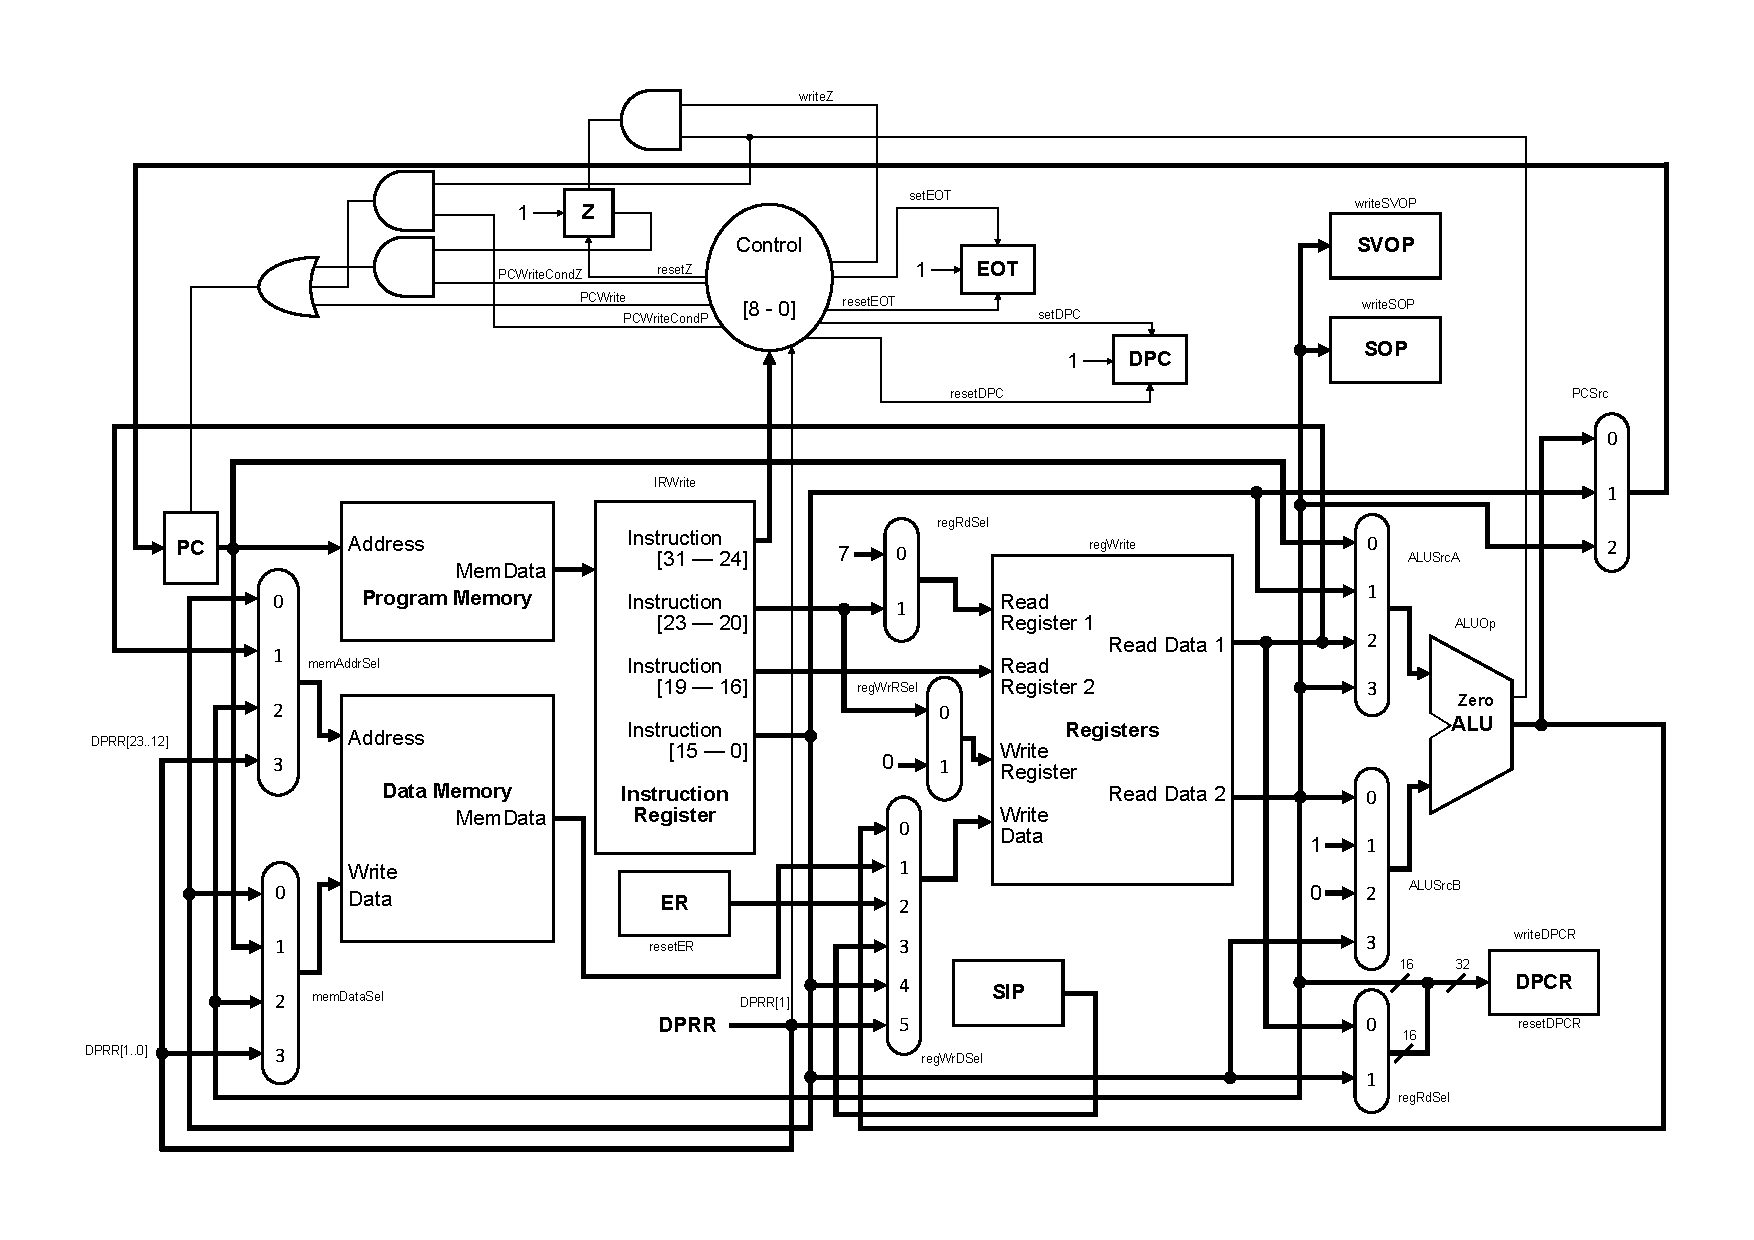
\includegraphics[clip, trim=0cm 1cm 0cm 1cm,scale=.85]{recop_datapath_harvard}%
		\end{adjustbox}
	\end{figure}
	
	
	
	\newpage
	
	\section{Application Specific Processor}
	Application Specific Processors (ASP) are hardware accelerators that specialise on very few number operations to significantly reduce the number of cycles that a general processor would otherwise require to do. \par
	An ASP was designed to accelerate a few arithmetic algorithms on arrays of data that would otherwise be performed on a JOP, including XOR, multiply and accumulate (MAC) functions, and average filter (AVE). The number of ASPs to be integrated into the network can be specified by changing the \texttt{num\_asp} in the top-level configuration file. \par
	As ASPs do not share memory with JOPs in the system, a JOP must send the data to the ASP’s internal memory using STORE command through the ASP Network Interface (ANI) and TDMA-MIN (see section \ref{sec:ani}). The particular ASP designed has 2 $N$-element ($N$ = 512 for this system) 16-bit vectors as data memory.
	
	\subsection{Control Unit}\label{header-c5}
	
	\begin{figure}[H]
		\centering
		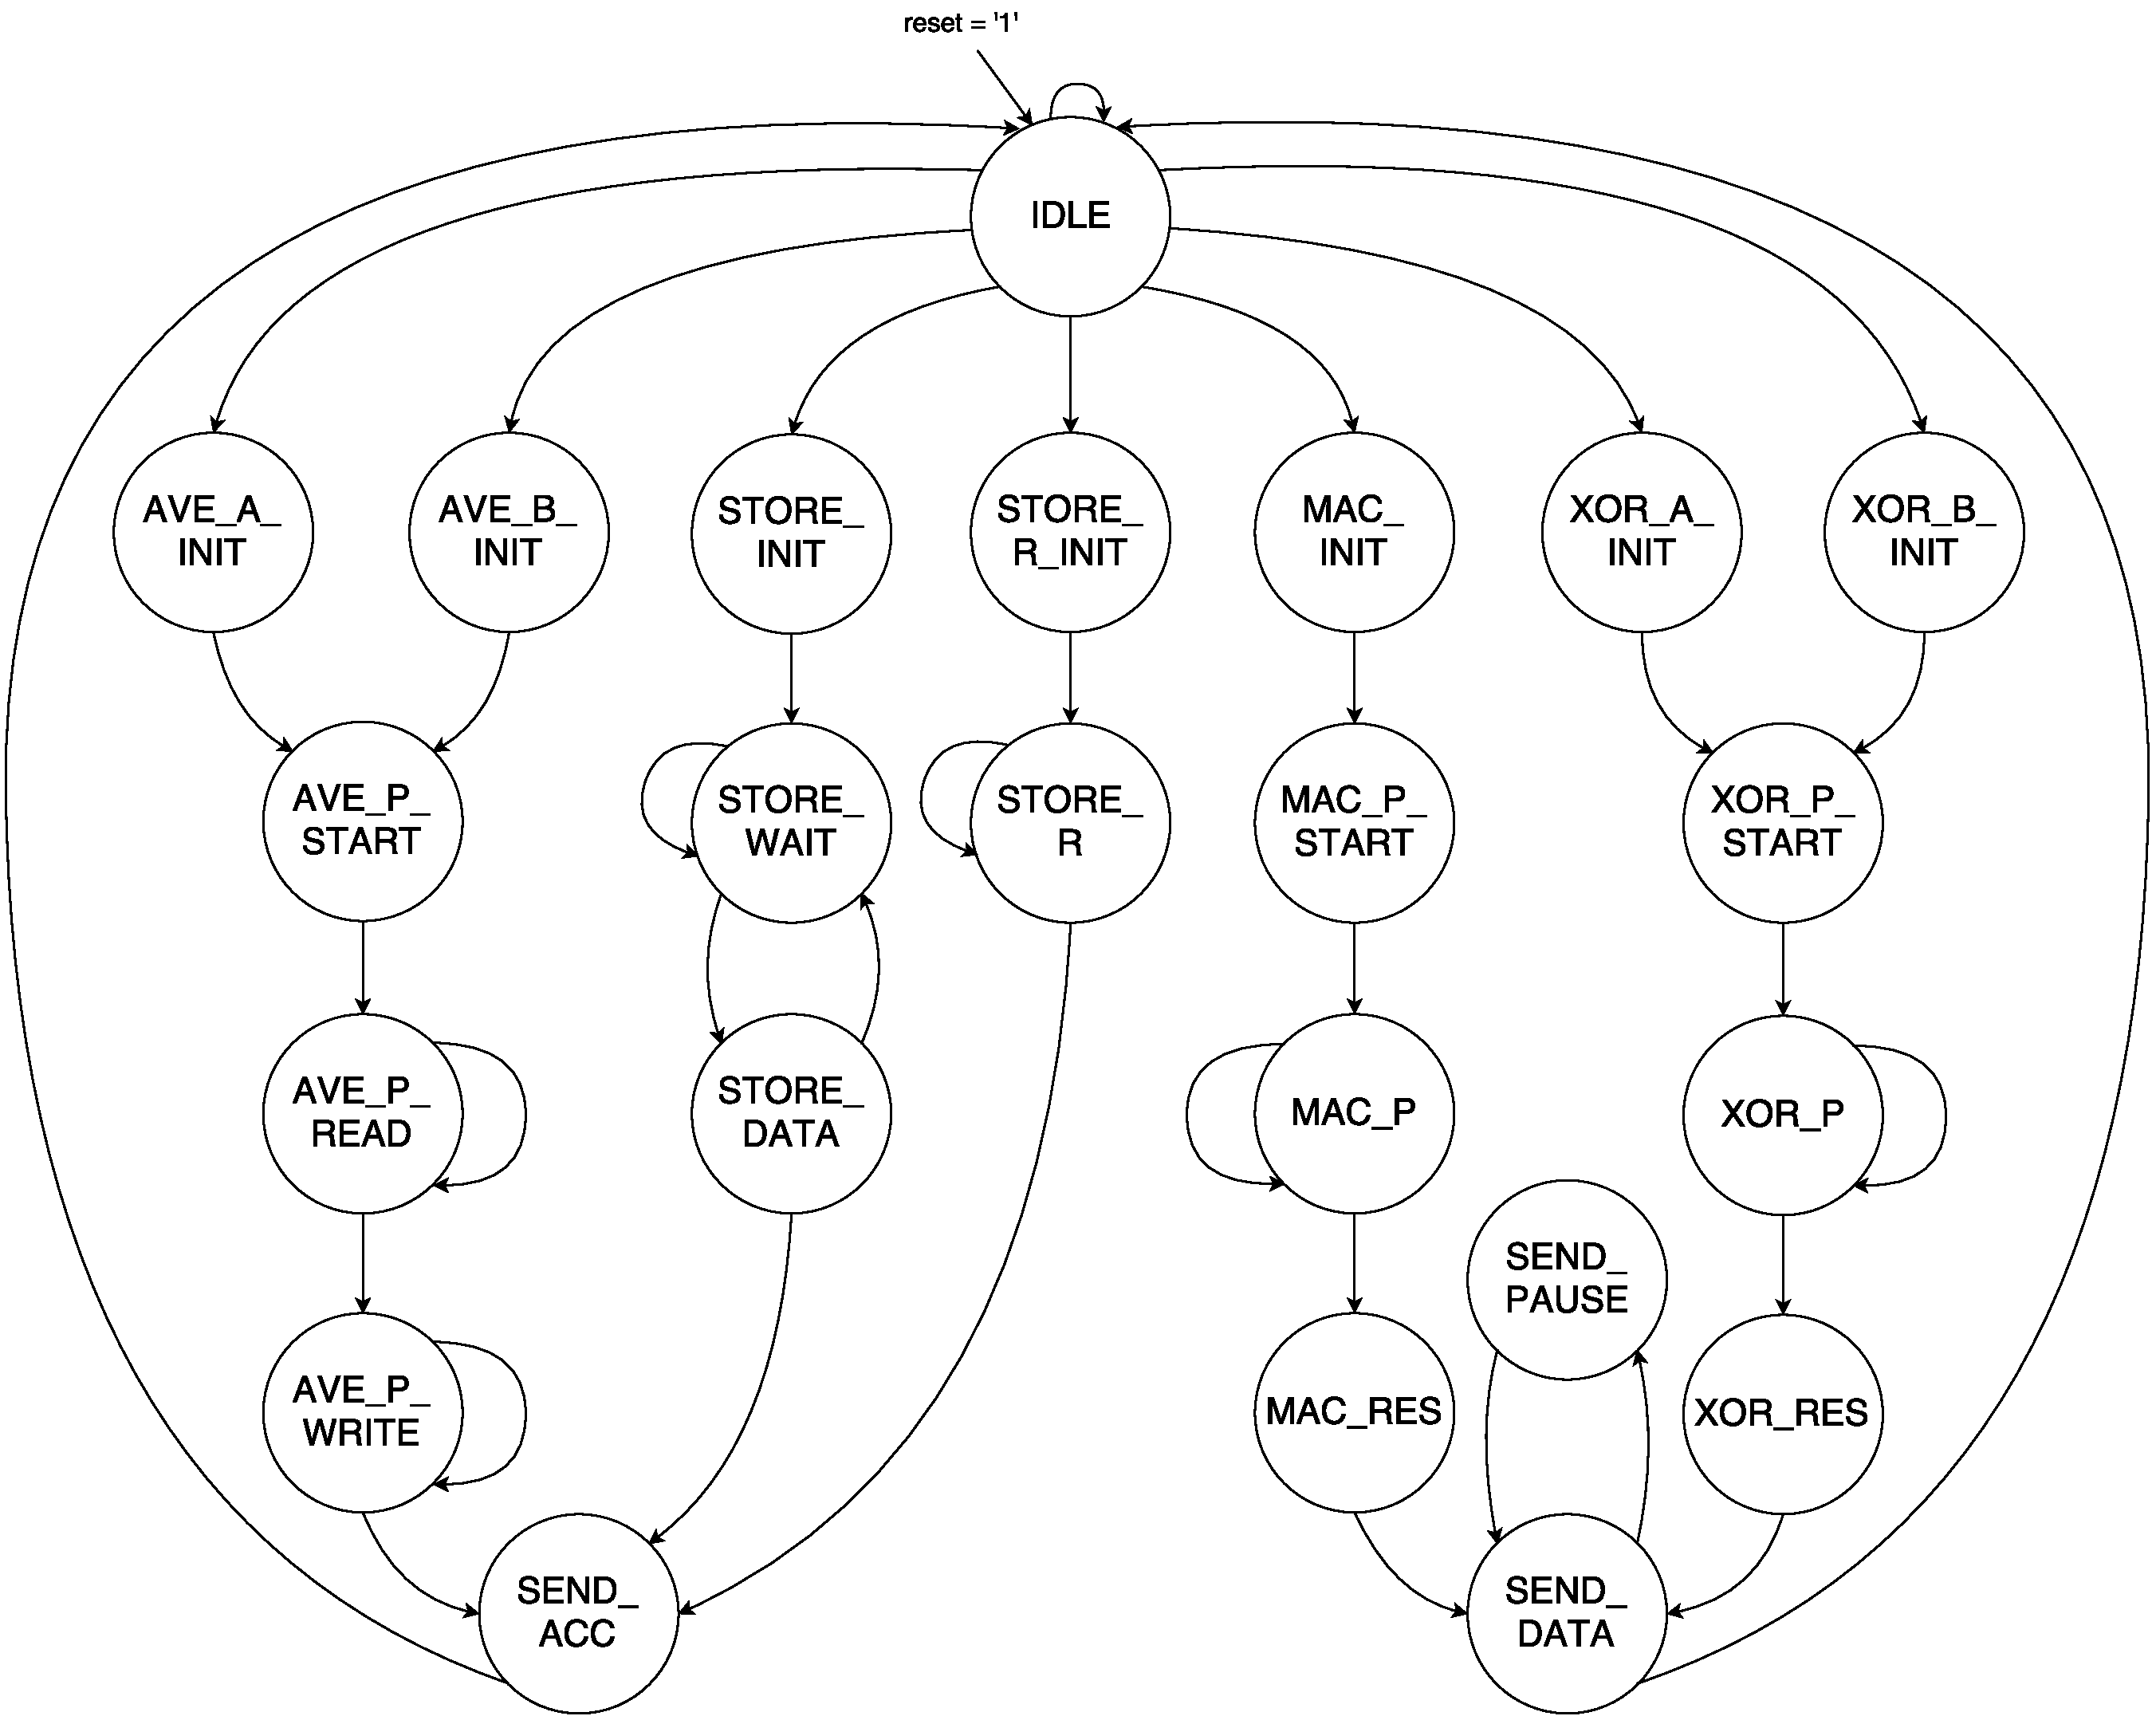
\includegraphics[width = 5.5in]{asp_fsm}
		\caption{ASP Control Unit FSM}
		\label{fig:asp_fsm}
	\end{figure}
	
	Control unit of the ASP uses the Moore FSM model to control the datapath in the system. ASP initialises in the \texttt{IDLE} state upon start up or if reset signal is high. \par 
	
	When the valid port is high, \texttt{d\_to\_asp} will be stored into ASP's internal register. If valid and legacy bits are 1's, a state transition depending on the op code will happen. All \texttt{INIT} states will clear result registers, initialises \texttt{rd\_pointer} and \texttt{wr\_pointer}. \par 
	
	Some operations require a stall cycle for the result registers to load before sending them, such as states \texttt{MAC\_RES} and \texttt{XOR\_RES}. There is also a one-cycle stall in the \texttt{SEND\_PAUSE} between each packet sent.
	
	\texttt{SEND\_ACC} sends \texttt{Operation Complete} packet.
	
	\newpage
	\enlargethispage{2in}
	\subsection{Datapath}
	
	
	\begin{figure}[H]
		\begin{adjustbox}{addcode={\begin{minipage}{\width}}{\caption{%
							ASP datapath.
						}\label{fig:asp_datapath}\end{minipage}},rotate=-90,center}
			\hspace*{-0.7in}
			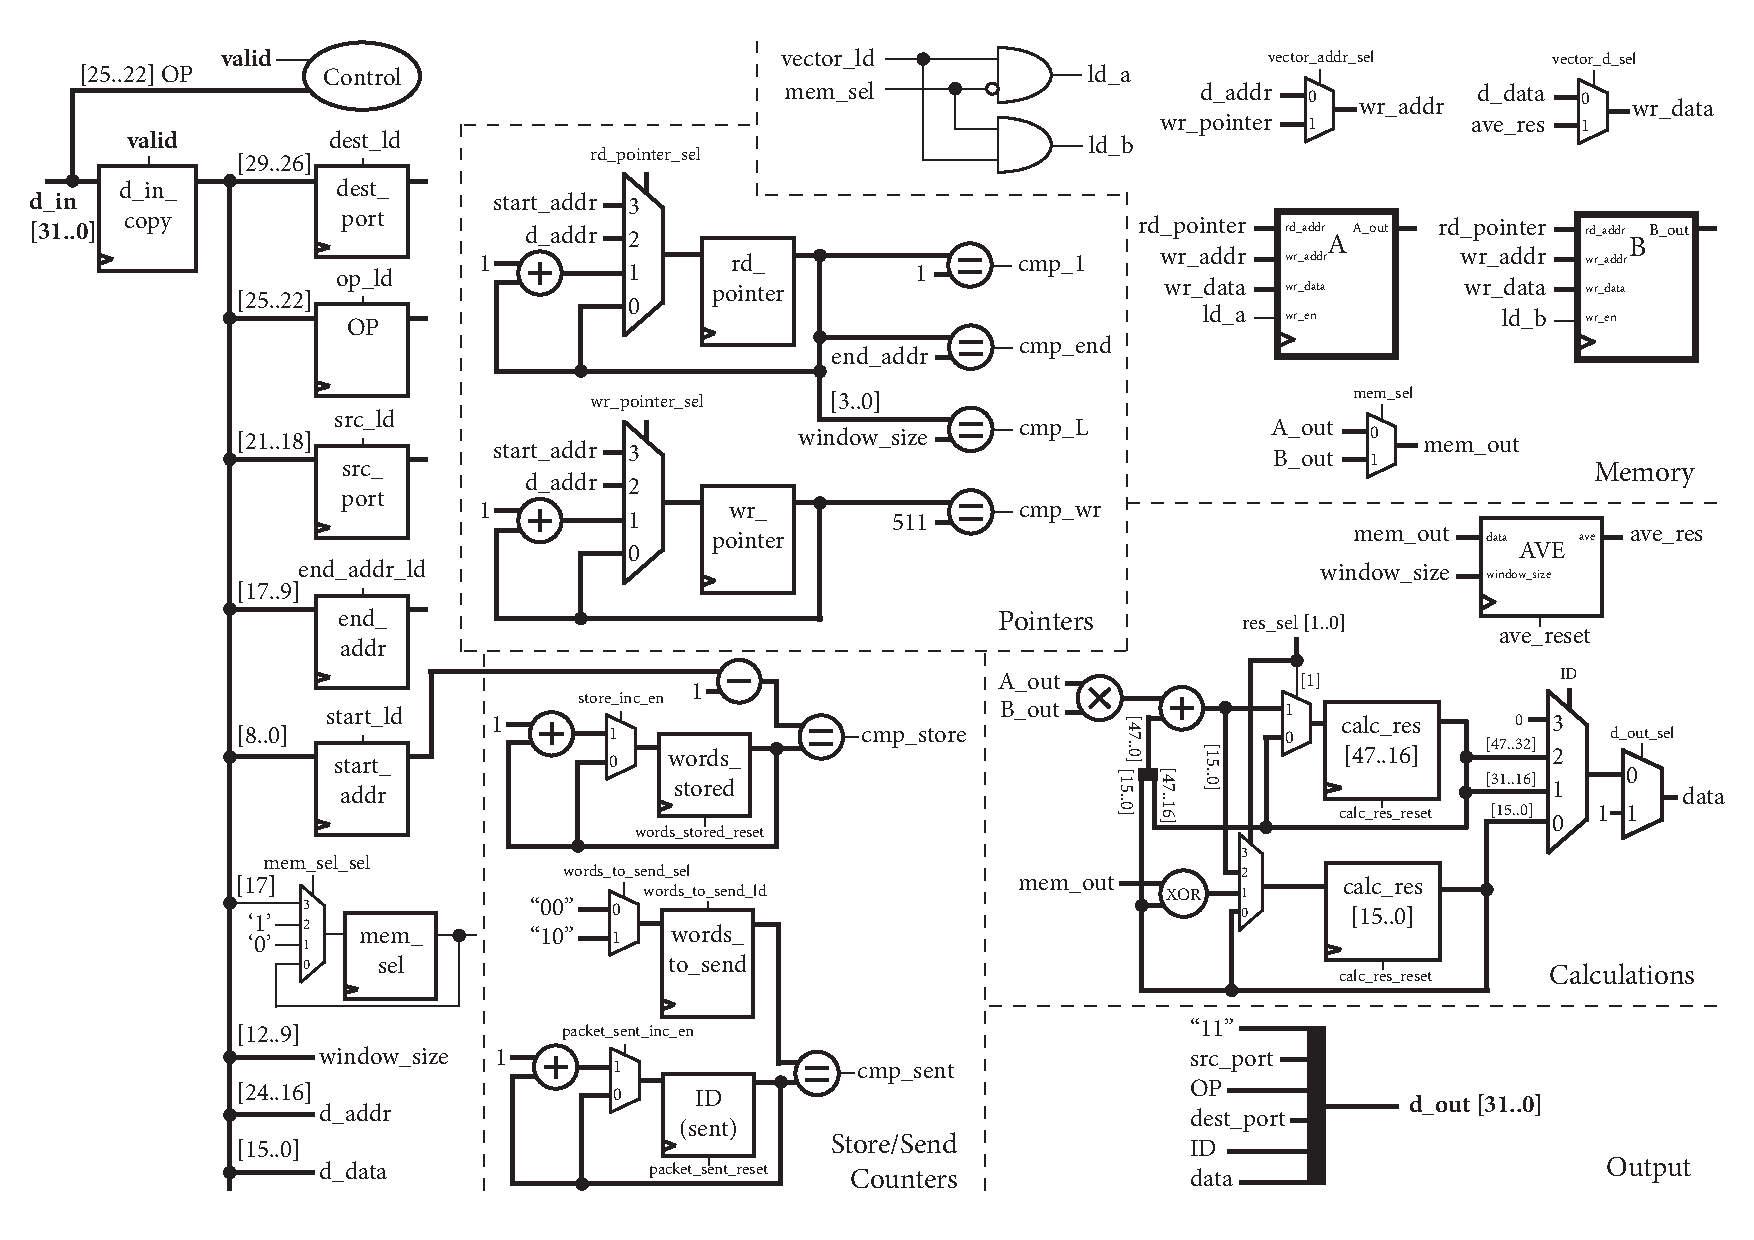
\includegraphics[scale=.8]{asp_datapath_v3}%
		\end{adjustbox}
	\end{figure}
	
	\newpage
	
	\begin{figure}[H]
		\centering
		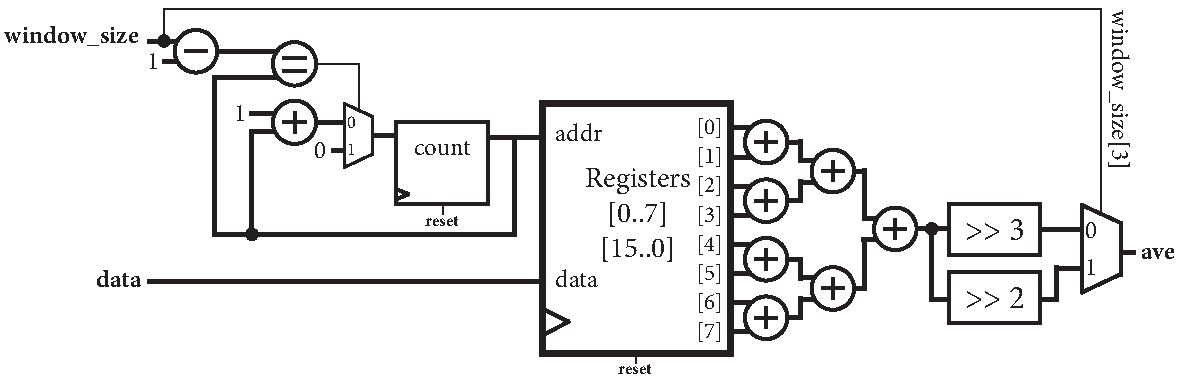
\includegraphics[width = 5.5in]{ave_filter_datapath}
		\caption{Average Filter datapath}
		\label{fig:ave_filter_datapath}
	\end{figure}
	
	\subsection{Operations}
	\subsubsection{Store Reset}
	Resets either vector A or vector B to 0 depending to the \texttt{mem\_sel} bit. An \texttt{Operation Complete} (formerly known as \texttt{Access Granted} packet -- 0x0001) will be sent back upon completion.
	
	$$T_{execution} = N + 2 \text{ clock cycles}$$
	
	\subsubsection{Store}
	This operation will store a fixed number of words to the ASP internal memory. It will send two types of packets -- a Store Invoke packet, followed by a series of Data packets (see section \ref{sec:asp_data_format}). The Store Invoke packet contains information on the number of words and which vector to be stored in. Data packets contain the 16-bit data and 9-bit address indicating the memory location to be stored at. The number of data packets must match the store invoke packet's specified number of words. Returns \texttt{Operation Complete}.
	
	$$T_{execution} = n_{words} + 2 \text{ clock cycles}$$
	
	\subsubsection{XOR}
	This function will perform a bit-wise XOR operation to the specified vector from index \texttt{begin\_address} ($m$) to \texttt{end\_address} ($n$) inclusively. After the operation, ASP will send the result to the back.
	
	$$T_{execution} = n - m + 3 \text{ clock cycles}$$
	
	\subsubsection{MAC}
	Multiply and Accumulate will perform a dot product opertion between index \texttt{m} to \texttt{n} for vector A and B. 
	\begin{equation}
	S = \sum_{i=m}^{n}A(i)B(i)
	\end{equation}
	There is a high probability that the MAC result will overflow a 16-bit data structure, with possible maximum being 41 bits.
	\begin{equation}
	(2^{16})^2 \times 512 = 2^{41}
	\end{equation}
	
	\par
	41-bit data can be sent as 3 packets of 16 bits. To stay consistent, the ASP will always send 3 packets consecutively. In order to differentiate between the packets, a 2-bit packet ID is inserted into each packet, from 0 to 2. ID 0 is the first packet and ID 3 being the last. It is up to the JOP programme to concatenate those 3 packets into a \texttt{long}.
	
	$$T_{execution} = m - n + 9 \text{ clock cycles}$$
	
	\subsubsection{AVE}
	Average filters vector A or B with a run-time window size (L) of 4 or 8 using the algorithm described in (\ref{eq:ave}). The datapath of the AVE block in Fig. \ref{fig:ave_filter_datapath} shows that the 8 internal registers are always summed and right shifted by 2 or 3 depending on the window size, and data is always stored at data registers at index \texttt{count}. The \texttt{count} is an up counter that resets after its value is \texttt{window\_size} - 1, as the register indexing is 0 to 7, while the \texttt{window\_size} can be 4 or 8. Bit 3 of \texttt{window\_size} is 1 when \texttt{window\_size} is 8, and is 0 otherwise, therefore it can be used as the select line of the output multiplexer to select between the right shift of 2 or 3 (divide by 4 or 8).
	
	\begin{equation} \label{eq:ave}
	X(i) = \sum_{k = i}^{i+L-1} \frac{X(k)}{L} \quad \text{where} \; i \in [0,N-L)
	\end{equation}    
	
	This allows pipelining, since it is always averaging a stream of data coming in, replacing the oldest. Upon initialisation, the registers are reset, \texttt{rd\_pointer} points at 0 and starts to increment by 1, \texttt{wr\_pointer} is set to point at 0, but not incrementing. When \texttt{rd\_pointer} is equal to the \texttt{window size}, the \texttt{AVE} registers will be filled, outputting the first average value, and \texttt{cmp\_L} will be high. The \texttt{cmp\_L} signal triggers a state transition, and \texttt{wr\_pointer} starts incrementing, and \texttt{vector\_ld} is set high in order to write into memory. This continues until the \texttt{rd\_pointer} overflows and equal to 1 -- when the element $N-L$ has been stored, which will then send \texttt{Operation Complete}.
	
	$$T_{execution} = N + 3 \text{ clock cycles}$$
	
	\subsection{Data Format}\label{sec:asp_data_format}
	
	\begin{figure}[H]
		\centering
		\captionsetup{justification=centering,margin=2cm}
		\begin{bytefield}[endianness=big,boxformatting={\centering},
			bitwidth=1em,bitheight=8.3mm]{32}
			\bitheader{0-31} \\
			\bitbox{1}{\rotatebox{90}{\tiny Valid}}
			\bitbox{1}{\rotatebox{90}{\scalebox{.5}{Legacy(1)}}} &
			\bitbox{4}{\small Dest} & 
			\bitbox{4}{\small OP code} &
			\bitbox{4}{\small Source} &     
			\bitbox{1}{\rotatebox{90}{\tiny memSel}} &
			\colorbitbox{gray}{8}{\small Unused} &
			\bitbox{9}{\small Number of words} & 
		\end{bytefield}
		\caption{Store invoke packet format to ASP}
		
	\end{figure}
	
	
	\begin{figure}[H]
		\centering
		\captionsetup{justification=centering,margin=2cm}
		\begin{bytefield}[endianness=big,boxformatting={\centering},
			bitwidth=1em,bitheight=8mm]{32}
			\bitheader{0-31} \\
			\bitbox{1}{\rotatebox{90}{\tiny Valid}}
			\bitbox{1}{\rotatebox{90}{\scalebox{.5}{Legacy(1)}}} &
			\bitbox{4}{\small Dest} & 
			\colorbitbox{gray}{1}{\rotatebox{90}{\tiny Unused}} &
			\bitbox{9}{Address} &     
			\bitbox{16}{Data} &
			
		\end{bytefield}
		\caption{Data packet format to ASP}
		
	\end{figure}
	
	
	\begin{figure}[H]
		\centering
		\captionsetup{justification=centering,margin=2cm}
		\begin{bytefield}[endianness=big,boxformatting={\centering},
			bitwidth=1em,bitheight=8mm]{32}
			\bitheader{0-31} \\
			\bitbox{1}{\rotatebox{90}{\tiny Valid}}
			\bitbox{1}{\rotatebox{90}{\scalebox{.5}{Legacy(1)}}} &
			\bitbox{4}{\small Dest} & 
			\bitbox{4}{\small OP code} &
			\bitbox{4}{\small Source} &     
			\bitbox{9}{\small End Address (inc)} &
			\bitbox{9}{\small Begin Address (inc)} & 
		\end{bytefield}
		\caption{Command invoke packet format to ASP}
		
	\end{figure}
	
	\begin{figure}[H]
		\centering
		\captionsetup{justification=centering,margin=2cm}
		\begin{bytefield}[endianness=big,boxformatting={\centering},
			bitwidth=1em,bitheight=8mm]{32}
			\bitheader{0-31} \\
			\bitbox{1}{\rotatebox{90}{\tiny Valid}}
			\bitbox{1}{\rotatebox{90}{\scalebox{.5}{Legacy(1)}}} &
			\bitbox{4}{\small Dest} & 
			\bitbox{4}{\small OP code} &
			\bitbox{4}{\small Source} &     
			\colorbitbox{yellow}{2}{\small \hl{\textbf{ID}}} &
			\bitbox{16}{\texttt{Data} or \texttt{OperationComplete}} & 
		\end{bytefield}
		\caption{Result packet format from ASP}
		\label{fig:yello_asp_packet}
	\end{figure}
	
	Due to the number of bits assigned to the destination port in ASP packet format -- 4 bits, the maximum supported nodes the ASP can communicate to 16 $(2^4)$. Each ReCOP and JOP takes a node in the network, therefore the maximum number of ASPs is 12, with 1 ReCOP and 3 JOPs.
	
	\section{ASP Network Interface} \label{sec:ani}
	In order for the ASP to communicate with the rest of the system, a network interface, ANI has been designed. The ANI contains two Altera Megafunction first-in-first-out (FIFO) queues to ensure all packets are sent and received. It is also responsible for sending packets during the correct TDM Slot Counter. \par
	
	\subsection{Datapath}
	
	\begin{figure}[H]
		\centering
		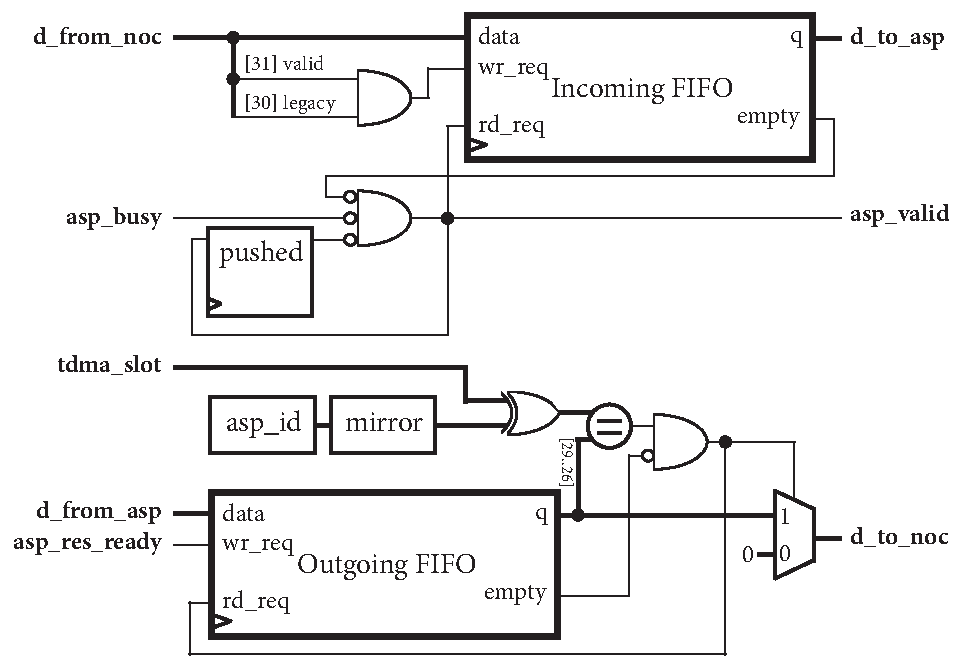
\includegraphics[width = 5in]{ani_datapath}
		\caption{ANI datapath}
		\label{fig:ani_datapath}
	\end{figure}
	
	ASP packets must have valid and legacy bits as 1's for pushing the packet from NoC into the Incoming FIFO. The head of the FIFO should only be popped to the ASP when it is not busy, not empty, and \texttt{pushed} as false. The \texttt{pushed} register makes sure that there is a one-cycle pause for the ASP to react to the previous packet before popping the next packet. \texttt{asp\_valid} is set to high when popping to indicate that new packet is to be processed in the ASP. \par
	
	When ASP has a packet ready to be sent to the NoC, it will have \texttt{asp\_res\_ready} high - this is used as the \texttt{wr\_req} to push the data packet to the Outgoing FIFO. For ANI to send the packet at the head to the correct port, the ANI's own assigned \texttt{asp\_id} is mirrored, XOR'ed and compared against the \texttt{dest\_port}.
	
	\subsection{Timing}
	
	\begin{figure}[H]
		\centering
		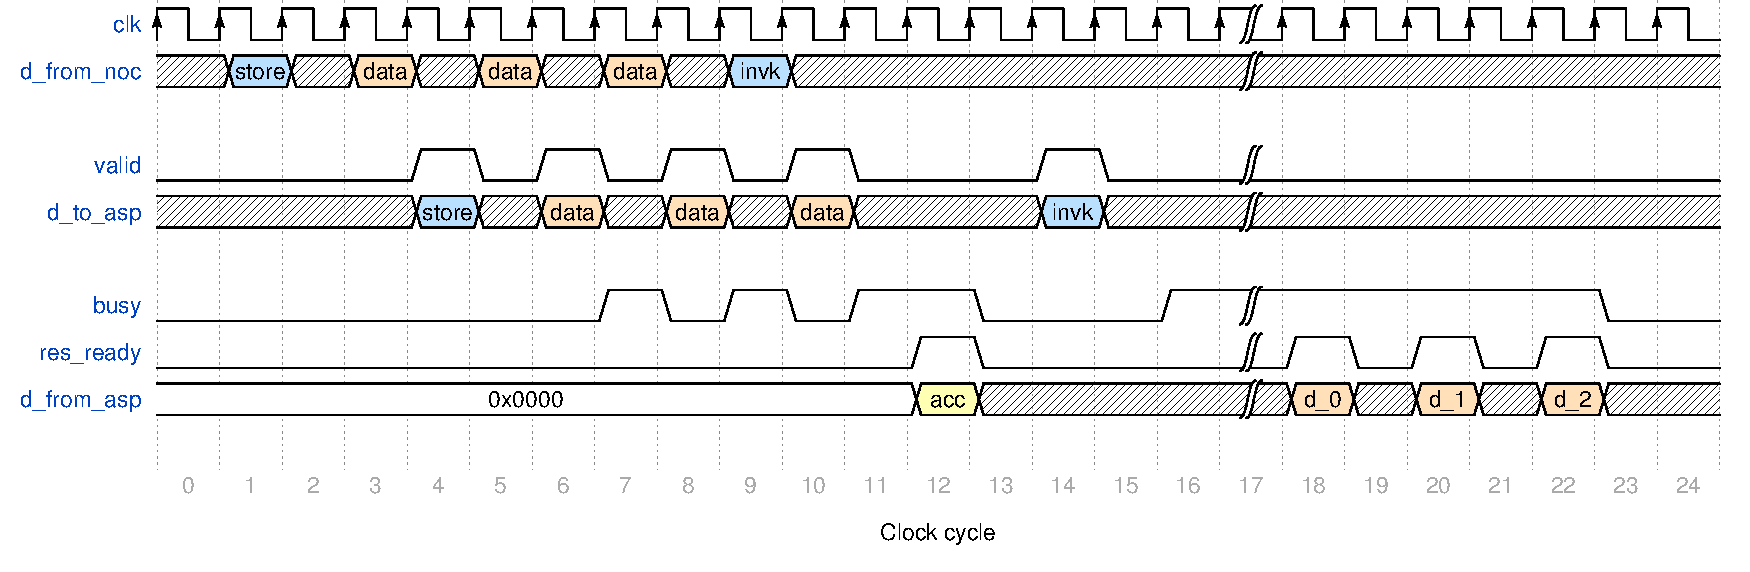
\includegraphics[width = 6.5in]{ani_timing}
		\caption{ANI timing with ASP}
		\label{fig:ani_timing}
	\end{figure}
	
	Fig. \ref{fig:ani_timing} shows the timings of packets from NoC and to NoC, \texttt{valid}, \texttt{busy} and \texttt{res\_ready} for Store 3 packets, followed by a MAC invoke command.
	
	
	\subsection{FPGA Testing}
	
	Both ASP and ANI were tested on the DE2-115 board during phase 1 of the project. The test bench consisted of:
	
	\begin{itemize}
		\item ASP
		\item ANI
		\item Fake JOP (emululates JOP ASP datacalls)
		\item Fake TDM Slot Counter
		\item BCD decoder for 7-segment display
		\item Switches and buttons from the environment
	\end{itemize}
	
	Upon a button press, Fake JOP reads the switches and send a packet or a series of packets hardcoded with ASP packets to the ANI's \texttt{d\_from\_noc} port. After command completion, the result packet from \texttt{d\_to\_noc} is transmitted to the BCD decoder and latched to be shown on the 7-segment display in hexadecimal format. This was when the ASP operation Store Reset was discovered to not be implemented -- fixed during phase 2.
	
	\newpage
	
	\section{JOP Network Interface}
	
	\begin{figure}[H]
		\centering
		\captionsetup{justification=centering,margin=2cm}
		\begin{subfigure}[t]{.55\textwidth}
			\centering
			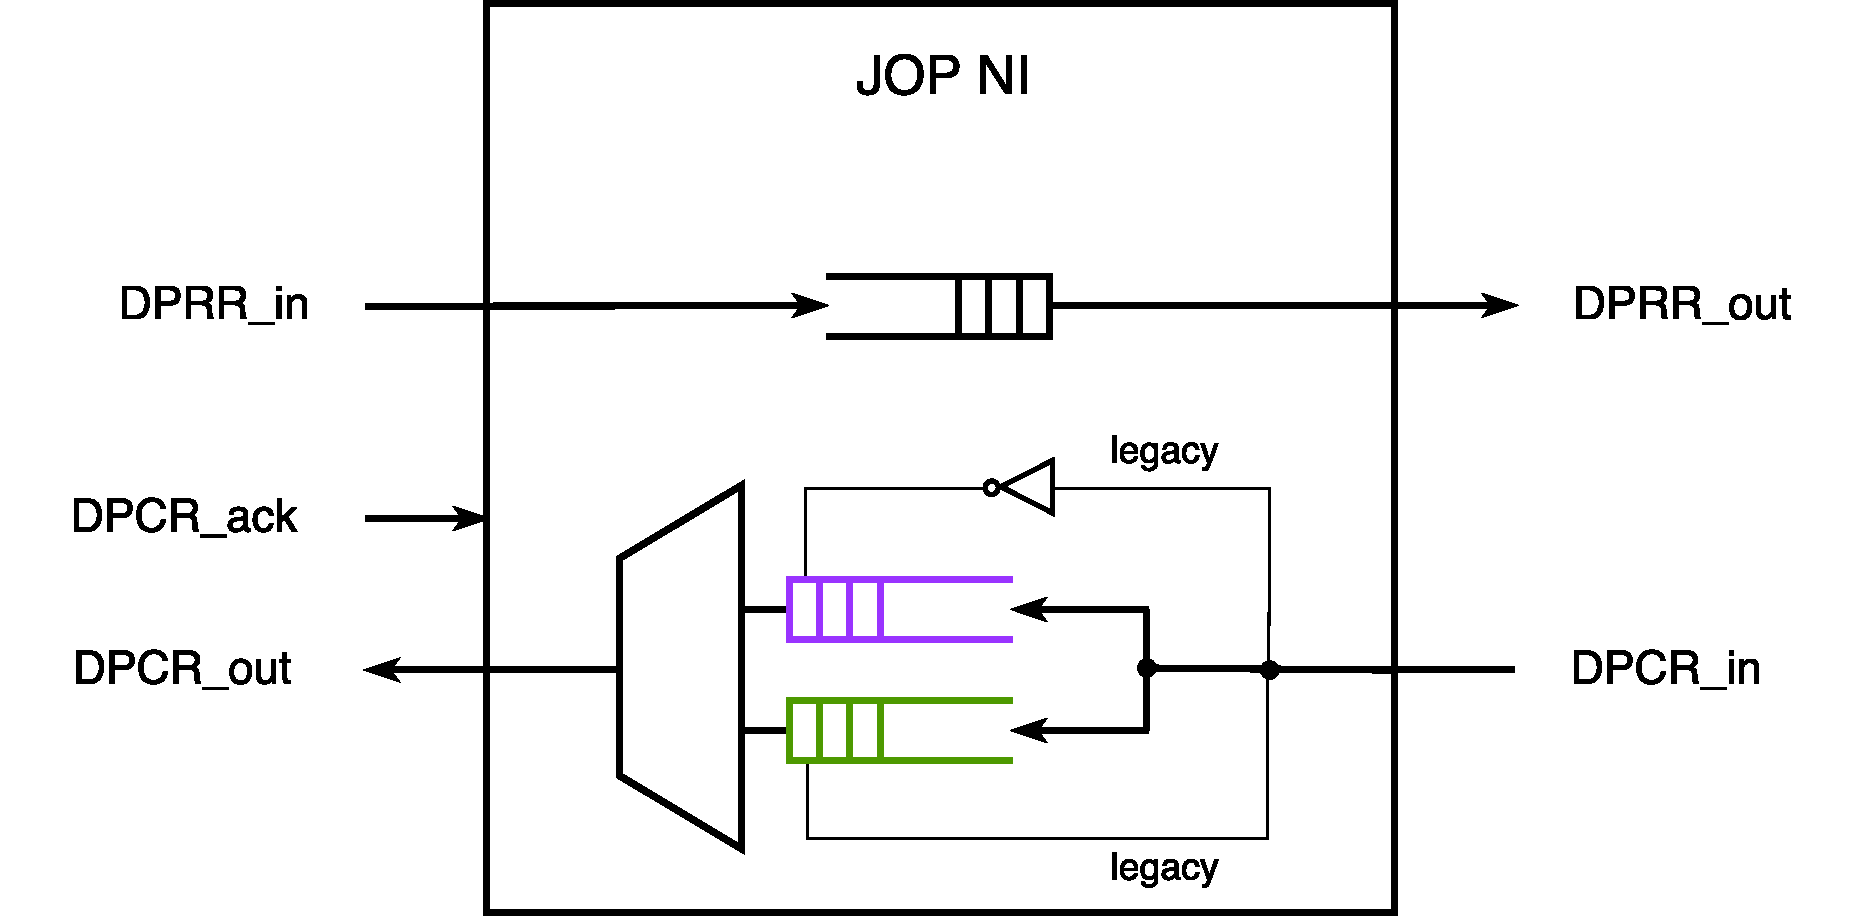
\includegraphics[width=3.5in]{jni_diagram}
			
			\caption{JNI Modifications}
			\label{fig:jni_diagram}
		\end{subfigure}%
		\begin{subfigure}[t]{.35\textwidth}
			\centering
			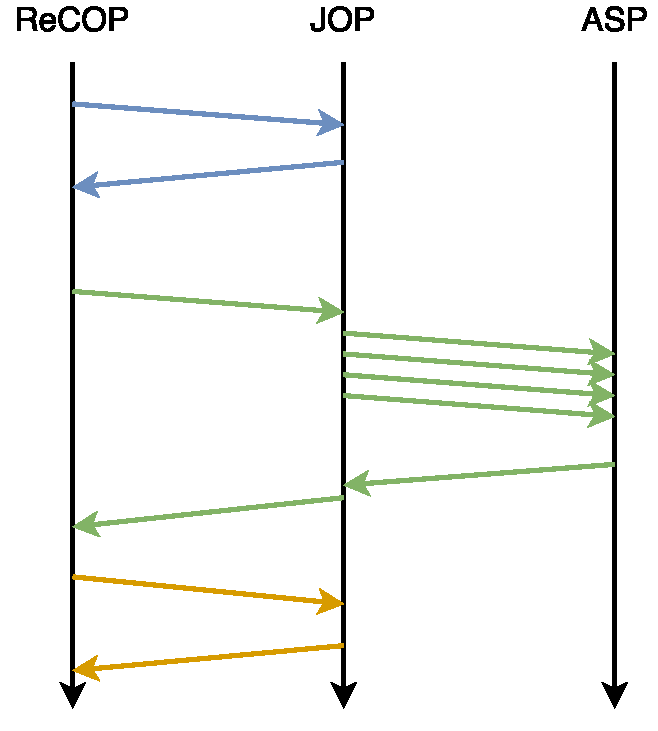
\includegraphics[width=1.7in]{rja_diagram}
			\caption{ReCOP, JOP and ASP communication sequence}
			\label{fig:rja_diagram}
		\end{subfigure}
		\caption{}
	\end{figure}
	
	
	For the communication of the JOP with ReCOP and ASP, lies an underlying protocol of communication. Whenever the ReCOP talks with the JOP, it can send data calls multiple times and the JOP responds with corresponding packets back to the ReCOP. Servicing each ReCOP datacall by the JOP will be slower than the how fast the ReCOP can send, so a FIFO is in place to capture the calls so that there is no loss of data packets. Invoking JOP to execute data nodes will or will not invoke the ASP and as a result, may or may not expect data coming from the ASP. An example of this can be seen in Fig. \ref{fig:rja_diagram}.
	\par
	
	
	As there are multiple inter-communications between ReCOP, JOPs and ASP there lies chance that packets read are from ReCOP but are expected to be from the ASP. To prevent this interleaving of data, some adjustments have been made to the JNI; this can be seen in Fig. \ref{fig:jni_diagram}. An additional FIFO will catch packets coming specifically from the ASP. The JNI will be able to aggregate the correct FIFO data to the JOP when there is an ASP invocation. How this is done is by checking any outgoing packets that are to be sent to the ASP, the data read by the JOP will now be switched to be reading from the ASP FIFO. Once the number of expected ASP packets have been received, the JOP will now be reading from the ReCOP FIFO.
	\par
	To check for outgoing packets for whether or not the packet is intended to be for ASP or ReCOP is done by checking the legacy bit. As coincidently the bit for ASP communication packets are set to be always one and ReCOP specific packets to be zero. If there were to be any changes to this, then the JNI would be modified to check for port mapping done at compile time. This would check if at the TDM slot was connected to an ASP or ReCOP port.
	\par
	Checking for the number of ASP packets to be expected is done by checking whether or not the outgoing packet is an ASP invoke packet. Depending on which instruction the ASP invoke is, will set the number of expected packets to be received, where all instructions receive one -- except MAC which is three. The checking of expected packets is not done with a counter comparison as one would expect, but with a comparison of the ASP packet ID (seeing Fig. \ref{fig:yello_asp_packet}), making it not require an ALU.
	
	
	\section{ReCOP Network Interface}
	\begin{figure}[H]
		\centering
		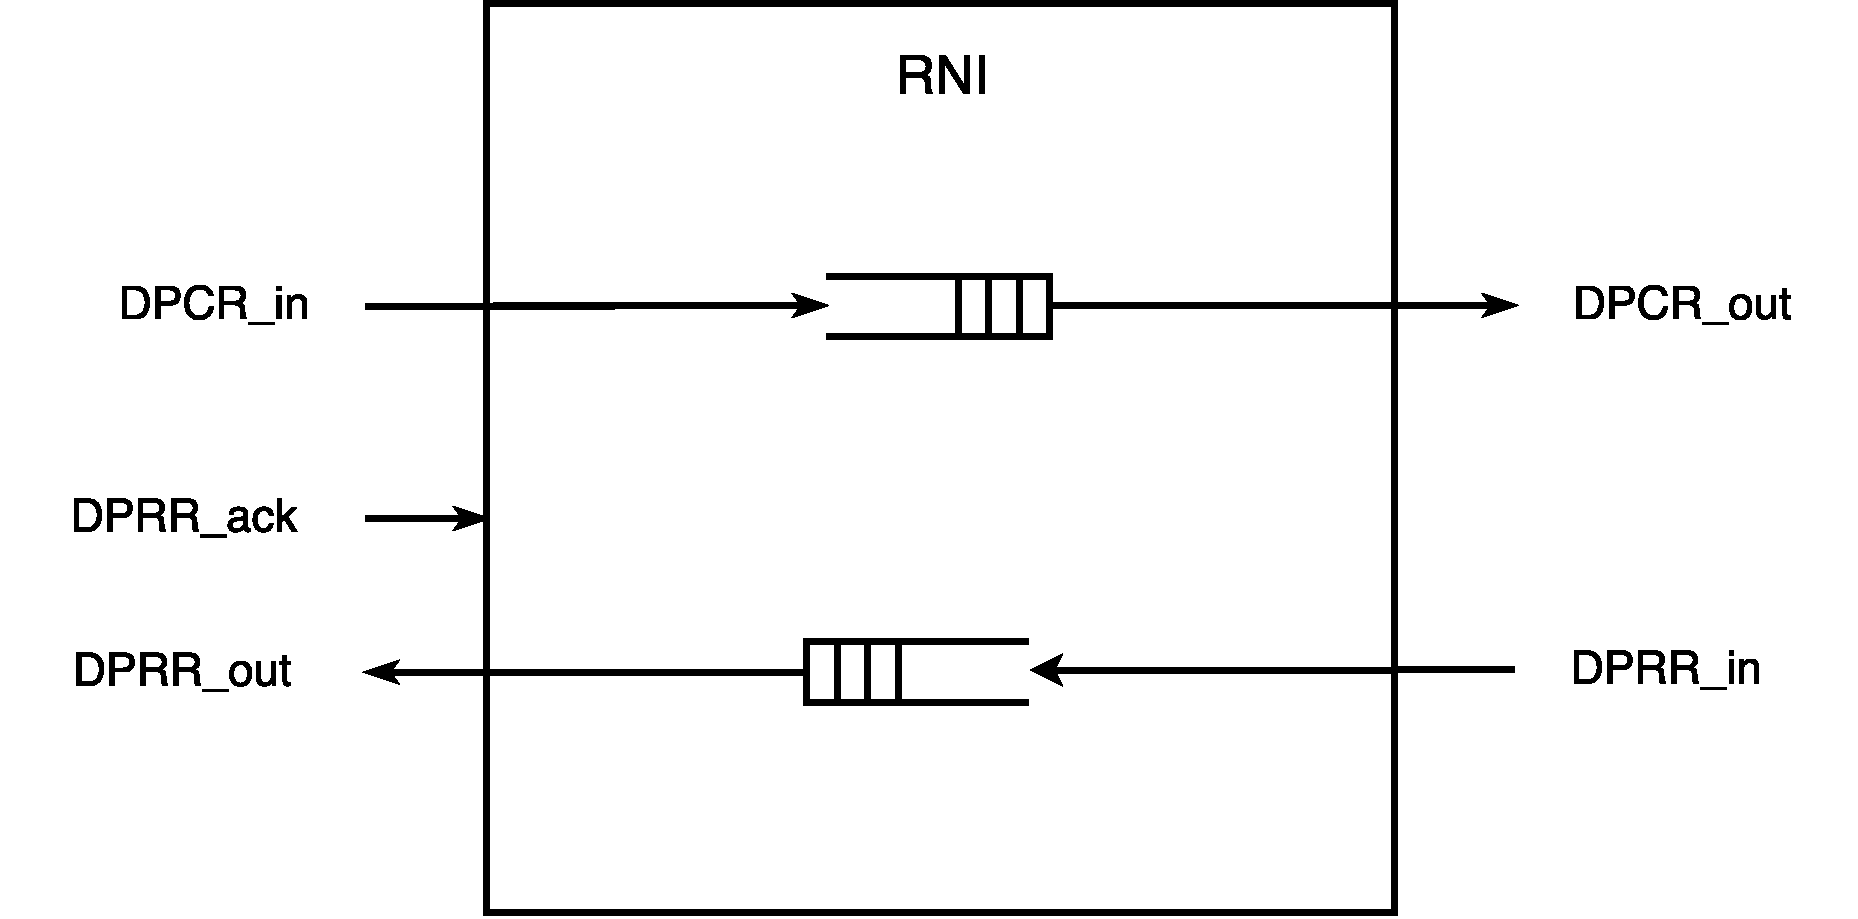
\includegraphics[width = 4in]{rni_diagram}
		\caption{RNI modifications}
		\label{fig:rni_diagram}
	\end{figure}
	
	The ReCOP\_AJS should in the current case of the ADD-HSoC, runs datacall result service routines at the end of each currently executed instruction, and as such does not interrupt its current instruction when a result from JOP is done. This can result in the fact that some packets from JOP can be missed on each TDM slot. The issue becomes is very apparent when there are one ReCOP and multiple JOPs in the system, where results from many JOPs may all quickly arrive and be overwritten. A small modification has been made to alleviate this issue by placing a DPRR FIFO to capture all the datacall results.
	
	
	\section{Java Programmes}
	
	\subsection{ASP APIs}
	\label{sec:java_api}
	Several APIs are provided in the \texttt{ASPCommunication} class. The developer has the responsibility of calling them using the correct \texttt{ASPid}, which specifies the ASP this packet is intended for. JNI will handle the correct ports, for the particular ASP ID. The number of ASPs is specified in the top-level configuration file. The list of APIs implemented is:
	\begin{enumerate}
		\item \texttt{private static void sendPacket(int packet);}\par
		Writes the packet to the data call result register, which will be sent to the JNI and out to the NoC. Used by the other public methods. Therefore this method cannot be used for sending packets to ReCOP directly. \par \par
		
		\item \texttt{public static int pollASPResponse();}\par
		Polls the datacall register. If \texttt{valid} and \texttt{legacy} bits are 1, the packet is returned. \par \par
		
		\item \texttt{public static int storeReset(int ASPid, int memSel);}\par
		Sends the reset invoke operation to ASP \texttt{ASPid} to reset vector indicated by \texttt{memSel}.This method returns the \texttt{Operation Complete} packet. Returns 1 upon completion. \par \par
		
		\item \texttt{public static int store(int ASPid, int[] data, int start, int memSel);}\par
		Sends a store instruction to ASP \texttt{ASPid} with an integer array. The instruction will store the array from \texttt{start} to \texttt{data.length} to vector specified by \texttt{memSel}. Returns 1 upon completion. \par \par
		
		\item \texttt{public static int xor(int ASPid, int memSel, int start, int end);}\par
		Sends an XOR instruction to ASP \texttt{ASPid}. The addresses of XOR instruction is from \texttt{start} to \texttt{end}. Returns the XOR result. \par \par
		
		\item \texttt{public static long mac(int ASPid, int start, int end);}\par
		Sends a MAC instruction to ASP \texttt{ASPid}. The addresses of MAC instruction is from \texttt{start} to \texttt{end}. It will poll response until 3 packets have been received and concatenated before returning the result.\par \par
		
		\item \texttt{public static int ave(int ASPid, int windowSize, int memSel);}\par
		Sends an AVE command to ASP \texttt{ASPid}. \texttt{windowSize} specifies the window size of the moving average filter -- must be 4 or 8. Returns 1 upon completion. \par \par
		
	\end{enumerate}
	
	All of the APIs listed above are blocking -- the programme will freeze until the ASP has responded with the expected number of packets. However, this can cause time predictability issues and greatly increase the tick duration, which is undesirable. A potential solution has been provided in Section \ref{sec:future_work}.
	
	
	
	
	\subsection{Multi-JOP Programme}
	
	A simple multi-JOP Java program was developed to perform a simple matrix multiplication:
	\begin{equation}
	\textbf{C} = \textbf{A} \times \textbf{B}
	\end{equation}
	\begin{equation}
	\textbf{A} = \begin{pmatrix}    2&3&5&2&3\\    3&2&3&4&1 \\ 2&3&1&2&3    \end{pmatrix}
	\quad
	\textbf{B} = \begin{pmatrix} 1&2 \\ 2&3 \\ 6&5 \\ 1&2 \\ 2&2 \end{pmatrix}
	\quad
	\textbf{C} = \begin{pmatrix} 46&48 \\ 31&37 \\22&28 \end{pmatrix}
	\end{equation}
	
	For the purpose of multi-JOP computation, each JOP will perform a row of matrix multiplication. Therefore for $JOP_i, i \in [0,2]$, the calculations it will perform are:
	\begin{equation}
	\sum\limits_{j=0}^{L}\textbf{C}_{ij} = \sum\limits_{k=0}^{N} \textbf{A}_{ki} \times \textbf{B}_{jk}
	\end{equation}
	Where $L$ is the number of columns of $\textbf{C}$, and $N$ is the number of columns of $\textbf{A}$. Notice the number of rows of $\textbf{B}$ is equal to $N$ as well.
	
	
	\section{Integration}
	In the final phase of the project, ReCOP\_AJS was successfully integrated with the SystemJ programmes. Multi-ASP support was also implemented, allowing the developer to specify the ASPid in the API call. The number of ASPs is specified in the config file and generated during compilation.
	\subsection{FPGA}
	\begin{table}[H]
		\centering
		\begin{tabular}{|c|c|c|c|}
			\hline
			\textbf{Entity} & \textbf{LE}    & \textbf{M9K} & \textbf{DSP} \\ \hline\hline
			1 ASP           & 484            & 2            & 2            \\ \hline
			1 ReCOP\_AJS    & 1113           & 72           & 0            \\ \hline
			3 JOPs          & 16643          & 283          & 0            \\ \hline
			ANI             & 95             & 2            & 0            \\ \hline
			RNI             & 8017           & 0            & 0            \\ \hline
			JNI             & 67182          & 0            & 0            \\ \hline
			MINoC           & 413            & 0            & 0            \\ \hline
			Misc            & 7              & 0            & 0            \\ \hline\hline
			\textbf{Total}  & \textbf{93954} & \textbf{359} & \textbf{0}   \\ \hline
		\end{tabular}
		\caption{Resource consumption on FPGA}
		\label{table:resource}
	\end{table}
	
	The complete system uses 82\% of the total available logic elements (LE), 83\% of M9K memory blocks on the DE2-115 board. Maximum operation frequencies were calculated by Quartus software using the Slow 1200mV 85$^0$C Model. 
	
	\begin{itemize}
		\centering
		\item $F_{\text{NoC\_MAX}} = 66.8 MHz$
		\item $F_{\text{ReCOP\_MAX}} = 72.0 MHz$
		\item $F_{\text{ASP\_MAX}} = 78.4 MHz$
	\end{itemize}
	
	The critical path in the system is in the JOPs, therefore it is difficult to improve the current system clock frequency of $60 \text{MHz}$.\\
	
	
	
	\subsection{Performance Analysis}
	\begin{table}[H]
		\centering
		\begin{tabular}{|c|c|c|c|}
			\hline
			\textbf{Operation (data size)}  & \textbf{JOP (us)} & \textbf{ASP (us)} & \textbf{Speedup factor (2 sf)} \\ \hline \hline
			XOR (64)    & 53       & 11       & 4.8     \\ \hline
			XOR (128)   & 101      & 12       & 8.4     \\ \hline 
			XOR (256)   & 197      & 14       & 14      \\ \hline
			XOR (512)   & 543      & 18       & 30      \\ \hline\hline
			MAC (64)    & 169      & 24       & 7.0     \\ \hline
			MAC (128)   & 332      & 24       & 14      \\ \hline
			MAC (256)   & 659      & 26       & 25      \\ \hline
			MAC (512)   & 1311     & 30       & 44      \\ \hline\hline
			
			AVE (512, $L=4$) & 18145    & 18       & 1100    \\ \hline
			AVE (512, $L=8$) & 19706    & 18       & 1100    \\ \hline
		\end{tabular}
		\caption{Performance comparison between JOP and ASP, including communication time.}
		\label{table:performance_comparison}
	\end{table}
	
	Execution times shown in Table \ref{table:performance_comparison} were recorded time differences between the start of the API call and after receiving the results averaged 3 times -- therefore they include the time taken to write into the JOP datacall registers and communication time in the TDMA-MIN. Time stamps were retrieved from the microsecond program counter at memory location \texttt{IO\_US\_CNT}. \par 
	
	All supported ASP invoke operations were tested against a JOP using data sizes with increments of powers of 2, from 64 to 512 elements.
	
	\subsection{SystemJ Program}
	
	\begin{figure}[H]
		\centering
		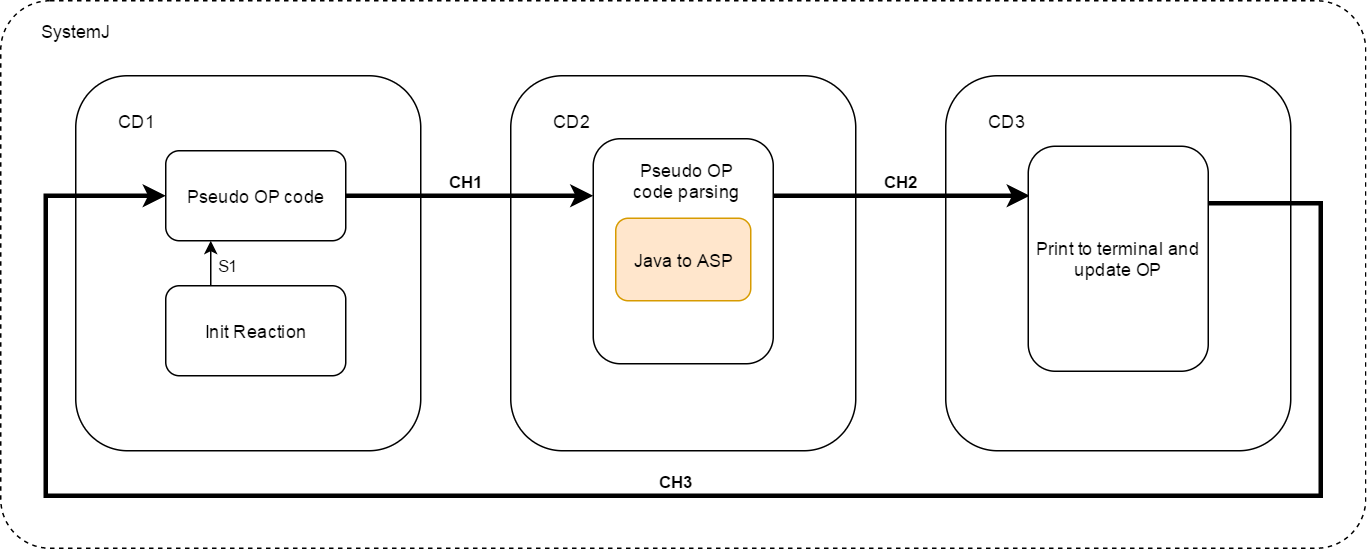
\includegraphics[width = 5.5in]{sysj_clock_domain}
		\caption{Clock-domain diagram for SystemJ program used}
		\label{fig:sysj_clock_domain}
	\end{figure}
	
	
	A SystemJ program was developed to showcase the ASP communication with AJS ReCOP in a multi-clock-domain (shown in Fig.\ref{fig:sysj_clock_domain}) scenario.  The SystemJ program is similar to the Java program which is showcasing the communications between ReCOP\_AJS, ASP and JOP. For SystemJ, one clock domain will be sending instructions to ASP after received an OP code from another clock domain. After the operation is completed on ASP and JOP receives the operation complete packet, this clock domain will send the opcode and result to the next clock domain to update the op code.
	
	\section{Future Work} \label{sec:future_work}
	Due to time constraints in the project, some aspects of the design were considered, but not implemented.
	
	\subsection{ReCOP}
	With the current nature of the multicycle implementation there lies possibility to expand the ReCOP functionality. The datapath has been laid out in a fashion where it is ready to be pipelined and it would be a simple process of sectioning each stage in the datapath into pipeline stages, as a result, the control unit will have to also accommodate for this future change. This will at least double the average number of instructions per cycle.
	
	\subsection{ASP}
	The memory blocks for vectors A and B can have two read ports. This can be used to parallelise some of the operations by having one read pointer going forward, starting at start address, and another read pointer going backwards, starting at end address until they rendezvous. This can reduce the execution time by up to half.
	
	\subsection{ANI}
	The current ANI design does not check whether the incoming packet has been delivered to the correct node in the network, which can be a security or data hazard. One potential fix is to compare the destination port within the packet against the ANI's assigned port number before pushing it into the incoming FIFO.
	
	\subsection{Java API}
	As mentioned in Section \ref{sec:java_api} the APIs are blocking. A possible fix is to create an ASPCommunication object to store the current progress of the datacall. When storing data, the complete array can be divided into smaller arrays by keeping track of the indices and only send one smaller block per tick. While waiting for a response from ASP, instead of blocking poll, call a separate method responsible for polling, checks the OP code in the response packet, concatenate the result if necessary then return it. Since ASP never return values larger than $2^{41}$, any values larger can be treated as \texttt{result not ready}.
	
	
	
	\section{Conclusion}
	The project has undergone through some major breakthroughs in order to design all the components to construct a full-blown ADD-HSoC. The expected amount of progress for each phase were completed at scheduled times without any major obstacles. \par
	
	The end prototype from the project showed promising results using SystemJ programs which show the communication between different processor types in the Heterogenous Multiprocessor System. \par
	
	The Reactive Coprocessor designed by AJS featured in the ADD-HSoC is able to effectively take control of the SystemJ control logic. Approaches for the ADD-HSoC configuration and any future changes in the ADD-HSoC would result in a straightforward process. \par
	
	Application Specific Processor that was designed during this project showed significant performance improvements compared to the existing Java Optimised Processors for specific computational operations.\par
	
	A set of Java APIs for communication between JOP and ASP was developed for intuitive program development. As a result, the full overview of the ADD-HSoC project produced a fully functional platform for computer systems designers to easily develop SystemJ applications with impelling computation acceleration and efficiency.
	
	
	
	\section{Acknowledgements}
	The authors would like to thank Professor Zoran Salcic and Dr Morteza Biglari-Abhari for their lectures on RTL, processor, and system designs, Benjamin Tan, Nicholas Harvey for their continuous guidance and support on this project. The authors would also like to thank Dr Heejong Park for his guidance and support for existing portions of the project.
	
	
	\bibliography{refs}{}
	\bibliographystyle{IEEETran}
	
	
	
\end{document}

